\section{Experience-Driven Organizational Evolution}\label{sec:evolution}
The outer improvement process takes evaluated task evidence and a parent package as input, constructs candidate revisions, and retains the selected organization for subsequent tasks.

\subsection{Experience and attribution}
We represent the evidence associated with an evaluated execution as
\begin{equation}
e=(x_{\mathrm{id}},h_v,\gamma,\ell_{\tau},\ell_y,s,c,u,\iota),
\label{eq:experience}
\end{equation}
where $\gamma$ identifies the frozen evaluation context; $\ell_{\tau}$ and $\ell_y$ locate run evidence and deliverable resources; $s$ is a scorer vector; $c$ records resource consumption; $u$ records human intervention; and $\iota$ locates independent integrity review. This tuple joins the implementation's separate run, evaluation, resource, and review records; intervention time is an additional study measurement. Task and package identities make the evidence attributable to a particular revision.

The Evolution Lab divides improvement work among observation, failure analysis, experiment planning, candidate authoring, evaluation, integrity review, and recommendation roles. The failure analyst identifies a recurring procedural mismatch and links it to concrete runs. For the running example, the hypothesis is that obligations distributed across the writer instructions and quality skill need a more explicit local sequence where individual claims enter the report. A candidate elaborates the claim-to-result handoff procedure and its reference example. This attribution is a testable hypothesis, not a causal conclusion inferred solely from an LLM explanation.

\subsection{Candidate space and update policy}
A candidate $\mathcal O'$ must preserve the package's logical identity, declare a new version, and contain a substantive change. Let $\operatorname{Cap}(\mathcal O)$ denote the union of locally expanded capability references declared by its orchestrator and agents; let $\operatorname{Base}(\mathcal O)$ denote their base-role set. Same-package capability sets are expanded to member references; external references retain their encoded identity. The integrity relation requires
\begin{align}
\operatorname{Cap}(\mathcal O')&\subseteq\operatorname{Cap}(\mathcal O_v),
&
\operatorname{Base}(\mathcal O')&\subseteq\operatorname{Base}(\mathcal O_v),
\label{eq:capability}\\
F'|_{\overline{M}}&=F_v|_{\overline{M}},
&
M&=M(\mathcal O_v)\cup M(\mathcal O')\cup\{m\}.
\label{eq:frozen}
\end{align}
$M(\mathcal O)$ contains declared prompts, the package README and selector instructions, and eligible UTF-8 skill instructions, references, and examples. Here $m$ denotes the manifest path, handled as a mutable declaration. Equation~\ref{eq:frozen} requires both file-set equality and byte equality outside the two text closures and the manifest. Candidate validation additionally resolves declared prompt paths, workflow agents, and dependencies, and rejects cycles.

The representation admits four kinds of change: procedural text; redistribution of inherited capabilities; workflow dependencies; and the role roster. Figure~\ref{fig:specialization} develops a procedural candidate within a concrete professional specialization. The union constraint in Equation~\ref{eq:capability} is package-wide. A newly introduced role can receive a capability previously held elsewhere in the parent, so it is not a per-role non-escalation guarantee.

The released candidate author is instructed to edit procedural text:
\begin{equation}
\mathcal O'\sim
  \mu_{\phi}(\,\cdot\mid\mathcal O_v,\mathcal E_{\mathrm{dev}},H\,),
\label{eq:mutation}
\end{equation}
where $H$ is the attributed failure hypothesis. The intended text space $\mathcal S_{\mathrm{text}}(\mathcal O_v)$ fixes the role roster, topology, capability allocations, and declared resource paths. It permits eligible instructions and references and the descriptive manifest fields named by the released authoring policy: top-level name, label, and description; selector summary and selection guidance; and agent, workflow, and workflow-node labels and descriptions. These descriptions can affect selection and dispatch without changing the declared roles or edges. All other manifest fields are fixed except the version label. A prompt does not guarantee that every sampled proposal belongs to this space. The research arm therefore checks the realized diff against $\mathcal S_{\mathrm{text}}$ before admitting a candidate to its trials; rejected attempts still consume its budget. This arm-eligibility check is part of the experimental protocol, distinct from the broader production validator. Structural mutation is an extension supported by the representation and integrity interface, rather than an automatically explored operator in this configuration.

\subsection{Worked example: refining a claim handoff}\label{sec:worked}
Consider a development case in which an analyst publishes a corrected result after an earlier calculation, and a report incorporates a value from the earlier revision. The arithmetic in the corrected resource is sound, but the final numerical claim has the wrong evidential basis. This is an illustrative execution pattern for explaining candidate construction, not a reported experimental case. The current writer instructions already require exact analysis and review resources. The shared quality skill additionally requires claim identifiers, result-table coordinates, verification evidence, and a report model populated from accepted claims. The candidate therefore changes where and in what order these existing obligations are presented to the writer; it does not introduce the evidence contract itself.

The failure analyst first distinguishes competing explanations. The writer may have read an old resource; it may have read the correct resource but transcribed the wrong cell; or the report renderer may have consumed a stale report model. These explanations require different revisions. A run whose locators identify the accepted analysis but whose report-model claim points to a superseded table supports investigating the handoff procedure. A run whose model is correct but whose rendered document differs instead directs attention to the rendering path. The evidence narrows the candidate hypothesis; a fluent retrospective explanation alone does not identify the cause.

For the handoff hypothesis, the text candidate reorganizes those distributed obligations into a checklist placed at the writer's claim-construction step: open the accepted result; resolve the associated review; bind the claim to its table coordinate; and write the value together with its qualifications and unresolved limits. A companion example contrasts a corrected result with a superseded one using generic placeholders. This changes the presentation and point of use of the existing requirements, while preserving their underlying acceptance contract. The update retains the role roster, collaboration declarations, capabilities, and executable files. Its reusable content is the sequence of checks and the reference pattern, rather than a copied task answer or a task-specific source locator. Figure~\ref{fig:specialization} shows this relationship between specialization, evidence, and procedural revision.

The transfer hypothesis concerns the effect of that reorganization: tasks that require carrying revised quantitative evidence into a report should exhibit fewer result--report mismatches. The same procedure can also add retrieval and checking cost, cause excessive abstention when review evidence is partial, or distract from qualitative synthesis. Matched trials therefore examine contract satisfaction and resource use, and retention tasks include assignments for which the extra numerical procedure is irrelevant. If improvement occurs only on the development example, the evidence supports fitting that example rather than transferable organizational learning. If output correctness remains unchanged while checking cost rises, the revision can be valid and precisely attributable without being useful.

\begin{figure}[!t]
\centering
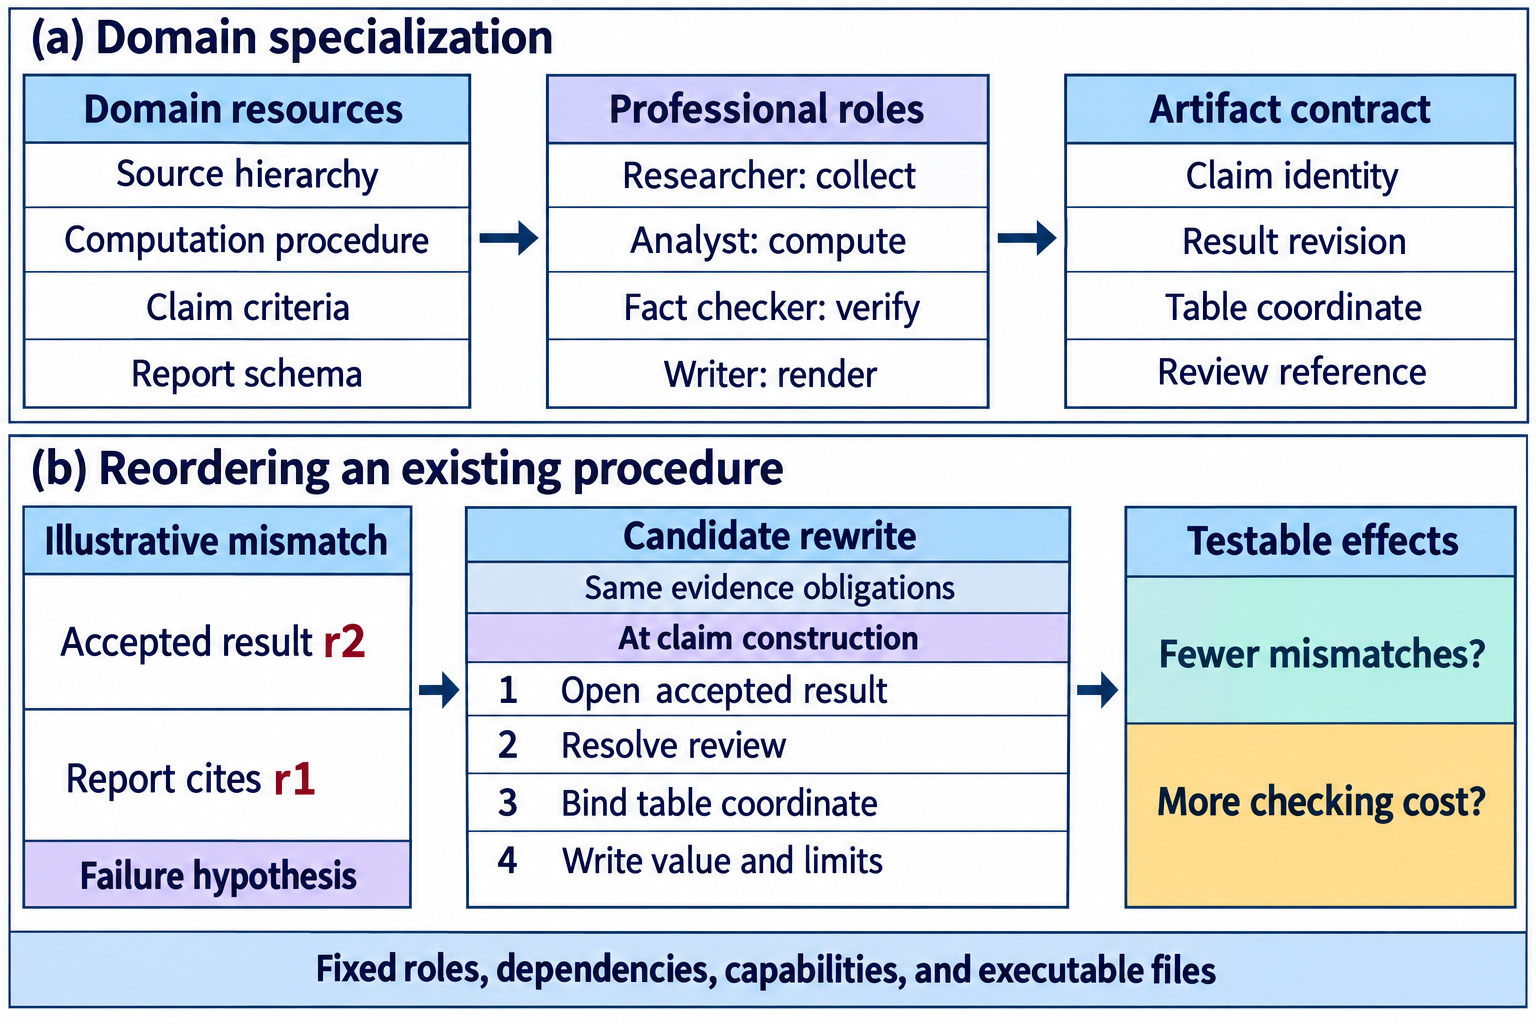
\includegraphics[width=\linewidth]{figures/specialization.png}
\caption{Domain resources and professional responsibilities support a shared analytical contract. The worked candidate reorganizes obligations already distributed across the writer prompt and shared quality skill into an explicit sequence at claim construction (Section~\ref{sec:worked}). The transfer hypothesis concerns this procedural reorganization; it does not establish a new evidence contract. The labels r1 and r2 denote illustrative superseded and accepted result revisions. The fixed-update footer describes the EEO--text research arm.}
\label{fig:specialization}
\end{figure}


\subsection{Matched comparison and retention}
A campaign fixes task cases, repetitions, scorer digests, model configuration, environment, permissions, arm order, and resource ceilings. Baseline and candidate executions occupy matched case--repetition slots and use their exact package revisions. The publisher derives candidate identities and file differences from validated resources. Evaluation results are projected from metric execution receipts, and independent integrity review binds to the exact evaluated revision.

For scorer $j$, let $s_{ij}^{a}$ be the value for slot $i$ and arm $a\in\{0,1\}$, with 0 denoting the parent. The comparison computes
\begin{equation}
d_{ij}=s_{ij}^{1}-s_{ij}^{0},\qquad
\bar d_j=\frac{1}{n}\sum_{i=1}^{n}d_{ij},\qquad
\widehat\Delta=\sum_j w_j\frac{\sigma_j\bar d_j}{|t_j-f_j|}.
\label{eq:comparison}
\end{equation}
Weights $w_j$ are the campaign's nonnegative weights normalized to sum to one, $\sigma_j\in\{-1,1\}$ sets the preferred direction, and distinct target and floor values $t_j,f_j$ define the scale. Missing required runs, scorers, or reviews make a comparison unavailable rather than contributing a zero score. The implementation reports paired summaries and an operational retain/select/inconclusive recommendation. Its multi-scorer interval approximation is discussed in Appendix~\ref{sec:implementation}; confirmatory inference uses the separate task-level analysis in Section~\ref{sec:analysis}.

Retention creates a traceable successor relation $\mathcal O_v\rightarrow\mathcal O_{v+1}$ and records the comparison context. Activation applies the selected revision to new tasks, preserving existing task bindings. A user-requested revision can also be retained through explicit feedback, but that path carries no claim of measured improvement. Selection, installation, and demonstrated learning therefore have distinct evidence.

Table~\ref{tab:algorithm} summarizes one complete improvement cycle. Candidate generation and matched comparison can repeat within the frozen development budget; the independent test partition is opened only after the final selection.


\begin{table}[htbp]
\centering\small
\begin{tabularx}{\linewidth}{@{}rY@{}}
\toprule
Step & One organizational improvement cycle \\
\midrule
1 & Freeze the parent package, development inputs, scorer versions, and total search budget. \\
2 & Inspect development run evidence; attribute a recurring failure and state a candidate hypothesis. \\
3 & Generate a text-policy candidate; check the realized diff for text-arm eligibility, then validate the package, inherited capabilities, and frozen files. Charge rejected attempts to search. \\
4 & Execute matched parent and candidate trials; collect metrics, failures, resource use, and independent integrity review. \\
5 & Record the comparison. Retain the parent or select an eligible candidate; keep each evaluated revision and its evidence addressable. \\
6 & Freeze the final selected revision before evaluation on unseen tasks and capability-retention tasks. Start later development with a fresh evaluation partition. \\
\bottomrule
\end{tabularx}
\caption{EEO improvement procedure. Steps 1--5 use Evolution Lab's package and evaluation interfaces. Step 6 specifies the research evaluation boundary; reuse of a test partition for subsequent candidate selection invalidates that boundary.}
\label{tab:algorithm}
\end{table}
